%!TEX root = ../Report.tex
\chapter{Software}
\section{软件实现流程}
\kaishu
\hspace*{5mm}软件内部实现的流程主要分为:\coloremph{初始化-硬件输入-程序执行-输出转化-硬件交互}。我们对于软件实现流程的流程图主要如下图所示:
\begin{figure}[htbp]
    \centering
    \caption{软件流程图}
    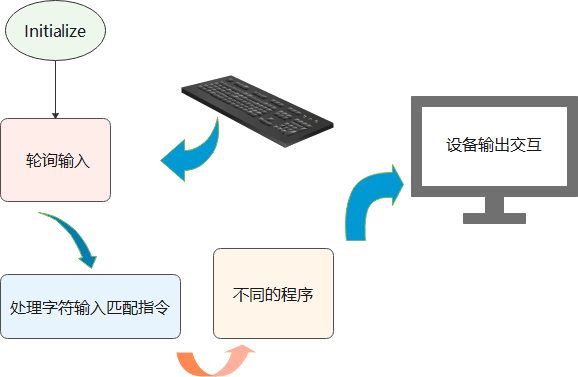
\includegraphics[scale = 0.5]{software.png}
\end{figure}
\songti
\\下面就分阶段地对软件的实现进行介绍。

\rule[-10pt]{14.3cm}{0.05em}
\subsection{软件内部信息初始化与约定}
\hspace*{5mm}这一阶段我们主要对一些寄存器进行清零操作,并确定特殊寄存器来存储固定的值,以供后续使用。
其中具有特殊功能的寄存器主要如下所示:
\kaishu
\\\hspace*{5mm}其中,\code{\$s3,\$s4,\$t9} 存储回车、换行、退格的ASCII码供键盘缓冲器判断使用;\code{\$t7} 存储1作为 \code{\$sp,\$gp} 执行过程中的增量(减量)。注意这里由于 \code{ROM} 生成的特点,\code{\$sp,\$gp} 取下一个值的增量为地址的1而非数据宽度4。 \code{\$t6} 存储`0'的ASCII码便于后续字符与操作数之间的转换。\code{\$s5} 存储的是VGA行,\code{\$s6} 存储的是VGA列。\code{\$sp} 是栈指针初始位置,\code{\$gp} 记录当前键盘输入的字符位置。
\begin{lstlisting}[style=assembler-style, caption={State Initialization}]
# 一些常数
addi $s3, $zero, 0x0d # 存储回车键
addi $s4, $zero, 0x0a # 存储换行键
addi $t9, $zero, 0x08 # 存储的是退格键
addi $t7, $zero, 1
addi $t6, $zero, 0x30 # '0'的ASCII码
# 特殊目的寄存器
add $s5, $zero, $zero
add $s6, $zero, $zero
addi $sp, $zero, 0x6000 # 一片空旷的,供栈空间使用的内存空间
add $gp, $zero, $zero # 键盘输入的字符
\end{lstlisting}
\hspace*{5mm}除此之外,我们对\code{HEX} 和\code{LED} 的初始值也通过对应寄存器传出指令进行了初始化,在打开开机界面前我们进行了VGA起始地址和须clear的屏幕的大小并调用刷新屏幕函数\code{\_clear\_screen},刷新后通过提供相应的字符开始位置和字符个数调用\code{\_print}函数显示欢迎界面。
\subsection{轮询硬件输入}
\songti
\hspace*{5mm}这里我们通过轮询键盘输入对特定输入进行检索并对应的跳转到其他函数处理。
\kaishu
\hspace*{5mm}首先是初始的\code{Press any key to continue},这里我们通过一个\code{\_wait\_loop}函数等待一个键盘输入,轮询到输入则进入到主页面并将该输入清除。
\begin{lstlisting}[style=assembler-style, caption={Wait for a key to continue}]
_wait_loop:
lw $a0, ($gp)
beq $a0, $zero, _wait_loop
sw, $zero, ($gp) # 进入主页面,将键盘RAM清零
\end{lstlisting}
\hspace*{5mm}进入主页面后通过\code{show\_prompt}函数显示命令提示符,进入\code{\_read\_key}函数中等待命令输入。这里将键盘输入存入缓冲区(\code{RAM}中的一块位置),处理时从缓冲区取出并对一些特殊的输入如shift,backspace进行特殊处理,检测到backspace则跳转至\code{\_Backspace}函数进行相应的清除工作(包括调整\code{\_write}写入VGA的字符和\code{\$gp}的内容与位置)后返回。对于其他字符,我们通过\code{\_write}函数写入VGA的\code{RAM}中,检测到回车键时跳转至\code{\_handle\_cmd}函数进行对应字符与命令的匹配和处理。
\hspace*{5mm}对键盘的轮询处理即\code{\_read\_key}函数如下所示。
\begin{lstlisting}[style=assembler-style, caption={Read and handle the key}]
_read_key:
lw $a0, ($gp)
beq $a0, $zero, _read_key
addi $t0, $zero, 0x10 # shift键
beq $a0, $t0, _read_key
beq $a0, $t9, _Backspace
add $gp, $gp, $t7
_handle_key:
jal _write
j _read_key
# 是Backspace开始处理
_Backspace:
beq $gp, $zero, _read_key # 在最开始,不能退回上一行了
add $a0, $zero, $zero # 退格相当于先退一格,然后在那个位置写上空白
sub $s6, $s6, $t7
add $s7, $zero, $t7
add $s7, $zero, $zero
sw $zero, ($gp)
sub $gp, $gp, $t7
sw $zero, ($gp)
j _read_key
\end{lstlisting}
\hspace*{5mm}其中\code{\_write}函数会将对应字符写入VGA的\code{RAM}中,该函数将在4.1.6节具体介绍。
\subsection{命令匹配过程}
\songti
\hspace*{5mm}我们将对应的命令字符事先存放在\code{RAM}中并对对应地址的字符与缓冲区中的键盘输入进行一一比对后跳转执行相应的子程序,未比对成功则默认跳转至相应函数调用\code{\_print}输出\code{Unknown Command}。
\\\kaishu
\hspace*{5mm}对应的我们编写了\code{\_strcmp}函数进行命令的比对,其中以回车键作为比较结束的标志。
\subsection{子程序的执行}
\songti
\hspace*{5mm}对于子程序的执行,我们大致分为两种,一种是无需进行操作数输入的:\code{hello, help, fail},其中\code{fail}是出现\code{Unknown Command}时调用的子程序;另一种是需要等待操作数的输入的:\code{fib, LEDon, LEDoff, display, piano}。\code{restart}作为特殊的子程序直接清空键盘缓冲器并回到初始化状态。
\kaishu
\\\hspace*{5mm}第一种,即直接进行信息输出,以hello为例,我们通过设置对应字符在\code{RAM}中的起始位置和字符数量直接调用\code{\_print}进行输出,由于无需等待操作数,输出后直接调用\code{main}等待下一个命令。
\begin{lstlisting}[style=assembler-style, caption={hello}]
_hello:
addi $a0, $zero, 0x1500
addi $a1, $zero, 196
jal _print
jal _cleargp # 打印的字符串里面有回车,不需要j _newline
j main # 等待下一个命令
\end{lstlisting}
\hspace*{5mm}第二种则分为两个阶段,第一个阶段进行命令的读入与匹配,保存命令号后继续调用\code{\_read\_key}读取操作数,根据命令号跳转至相应的函数处理操作数,其中\code{\_atoi}函数将把操作数输入时输入的字符转换为操作数,该函数将在4.1.5节具体介绍。
\\\hspace*{5mm}以\code{fib}为例,首先在\code{\_handle\_cmd}中通过\code{\_strcmp}匹配对应字符。
\begin{lstlisting}[style=assembler-style, caption={fib-judge}]
# fib
addi $a1, $zero, 0x1750 #fib命令在RAM中的起始地址
jal _strcmp
bne $v0, $zero, _fib_cmd # 设置s2=1
\end{lstlisting}
\hspace*{5mm}接着跳转至\code{\_fib\_cmd}函数进行命令号的设置(\code{\$s2}固定存储命令号,为0时表示无当前进行的命令),后通过\code{\_cleargp}清除缓冲区的字符命令,跳转至\code{\_read\_key}读入操作数(直接跳转至\code{\_read\_key}不调用\code{show\_prompt}展示命令提示符)。
\begin{lstlisting}[style=assembler-style, caption={fib\_cmd}]
_fib_cmd:
addi $s2, $zero, 1 # 置1等待参数
jal _cleargp
j _read_key
\end{lstlisting}
\hspace*{5mm}上层读到回车后再次回到\code{\_handle\_cmd}判断是否有命令号,有则跳转到\code{\_op\_handle}如下(其中如果判断没有输入操作数则继续调用\code{\_read\_key}读入),这里通过\code{\_atoi}进行输入字符向数字的转化,转化的数字参数存储在固定寄存器\code{\$t5}中:
\begin{lstlisting}[style=assembler-style, caption={\_op\_handle}]
_op_handle:
lw $t0, ($zero)
beq $t0, $s3, _void_op
jal _atoi
add $t5, $zero, $v0 # t5中存放参数
addi $t0, $zero, 0x1
beq $s2, $t0, _fib
addi $t0, $zero, 0x2
beq $s2, $t0, _piano
addi $t0, $zero, 0x3
beq $s2, $t0, _LEDon
addi $t0, $zero, 0x4
beq $s2, $t0, _LEDoff
addi $t0, $zero, 0x5
beq $s2, $t0, _hex
_void_op:
add $gp, $zero, $zero
sw $zero, ($gp)
j _read_key
\end{lstlisting}
\hspace*{5mm}通过判断命令号跳转到相应的子程序处理操作数(这里是\code{\_fib}进行Fibonacci数的计算),计算后通过\code{\_itoa}进行数字向字符的转化后调用\code{\_print}输出对应的结果。
\begin{lstlisting}[style=assembler-style, caption={Calculation of Fibonacci number}]
_fib:
add $t0, $zero, $t5  # 数字参数在t5里
add $t1, $zero, $zero
addi $t2, $zero, 0x1
xor $t3, $t3, $t3
_fibo_loop:
beq $t0, $zero, _fido_ret
sub $t0, $t0, $t7
add $t3, $t2, $t1
add $t1, $zero, $t2
add $t2, $zero, $t3
j _fibo_loop
_fido_ret:
add $v0, $zero, $t1
add $t5, $zero, $v0
add $a1, $zero, $zero
jal _itoa
addi $a0, $zero, 0x2000 #从2000开始打印
jal _print
jal _newline
j main
\end{lstlisting}
\hspace*{5mm}执行完成后回到\code{main}中清空命令号和操作数寄存器\code{\$s2, \$t5}并调用\code{show\_prompt}输出命令提示符,继续轮询键盘输入判断字符。
\subsection{输入输出间形式的转换}
\songti
\hspace*{5mm}如上节所述,处理操作数的子程序需要将对应的字符转换为对应的数字,处理后需要将数字转换为字符写入VGA的\code{RAM}中,所以我们分别提供了\code{\_atoi}和\code{\_itoa}的汇编代码进行输入输出形式之间的转换。
\kaishu
\\\hspace*{5mm}说明:这里为了处理的方便,我们规定输入输出均为十六进制数。
\subsection{与硬件之间的交互}
\songti
\hspace*{5mm}上述过程主要描述了软件内部工作原理,与硬件输入之间的交互则通过轮询键盘输入地址寄存器\code{\$gp}中的值取得键盘输入缓冲器中的值并进行对应的处理。
\\\hspace*{5mm}而与硬件输出的交互主要包括:VGA字符显示,LED的输出,HEX的显示和piano的播放。
\kaishu
\\\hspace*{5mm}字符的显示由\code{\_print}(输出既定起始位置开始既定数量的字符)和\code{\_write}(输出一个字符)完成。换行操作由\code{\_newline}完成,屏幕的滚动通过\code{\_moveon}完成。
\\\hspace*{5mm}LED的输出,HEX的显示,piano的播放均通过在硬件中判断命令号寄存器\code{\$s2}的值和操作数寄存器\code{\$t5}的值进行对应的处理以输出显示。
\songti
\\\hspace*{5mm}除此之外,在处理键盘缓冲区字符时,也需要与硬件的合理交互。
\kaishu
\\\hspace*{5mm}具体地,需要每次处理命令后将键盘缓冲区地址\code{\$gp}清零并将缓冲区字符通过\code{\_cleargp}函数清空,为下次命令字符的读入做准备。
\section{遇到的问题和解决方法}
\subsection{寄存器约定与协调}
\subsection{程序之间的协同}
\section{得到的启示}
